\section{Introdução}

Quando um volume de líquido é injetado dentro do vítreo, como no caso do procedimento de injeção intravítrea (IVI), há um aumento repentino da pressão intraocular (IOP), seguida de uma posterior adaptação que traz o sistema novamente ao valor basal após alguns minutos. O presente relatório constrói um modelo de zero dimensões na tentativa de reproduzir essa resposta a partir do balanço de volume. 

O olho pode ser tratado como uma cavidade fechada de volume variável $V$, cuja pressão interna $P(V)$ depende do volume por meio de uma curva de rigidez própria do tecido ocular. O volume se altera conforme líquido entra e sai pelas diferentes vias, cada uma delas descrita por um termo de vazão.

O objetivo do modelo é permitir que se calcule, a partir de parâmetros anatômicos e fisiológicos, a curva $\mathrm{IOP}(t)$ que resulta de uma IVI. O modelo é propositalmente simples para que, se validado, possa ser operado sem simulações computacionais robustas. 

Sua utilidade está em capturar, com poucos parâmetros, a escala de tempo e a magnitude, servindo de esqueleto sobre o qual dados experimentais e clínicos podem depois ser encaixados.

\section{Geometria e a hipótese de casca fina}
\label{sec:geometria}

A deformação da parede ocular, principalmente relacionada à esclera, é um fator importante na relação entre a pressão e o volume do olho. Quando essa parede é fina o suficiente em relação ao raio interno da cavidade, pode-se descrever a sua resistência à deformação de forma integral pelo esticamento da parede, sem a necessidade de considerar a flexão \citep{timoshenko1959}, permitindo obter uma fórmula para a rigidez ocular, ao invés de recorrer a um modelo numérico completo.

Para que a hipótese de casca fina possa ser aplicada, é necessário que a razão entre o raio $R$ e a espessura $t$ da parede seja maior do que 10 \citep{timoshenko1959}. Em um olho humano, com raio médio de $\SI{12}{\milli\meter}$ \citep{moosajee2023} e esclera de espessura média $\SI{0{,}5}{\milli\meter}$ \citep{vurgese2012}, a razão $R/t$ gira em torno de $24$. No olho de coelho, com raio médio de $\SI{7{,}6}{\milli\meter}$ \citep{bozkir1997, missel2012, lamminsalo2018} e espessura da esclera de $\SI{0{,}33}{\milli\meter}$ \citep{missel2012, zhang2014cxl, lamminsalo2018}, a razão $R/t$ é em torno de $23$. As duas espécies se situam, portanto, dentro de uma faixa em que a hipótese de casca fina é adequada. Ambas as espécies ainda apresentam valores de $R/t$ muito próximos entre si, indicando possivelmente que a diferença de rigidez observada nos estudos realizados com ambas as espécies não é dominada pela proporção entre raio e espessura, mas sim pela diferença de escala absoluta do globo.

A esclera não é uma estrutura uniforme. Sua espessura varia entre regiões do globo ocular e entre espécies \citep{vurgese2012,olsen1998,prince1960}. O valor de $t$ no modelo é uma média regional. O olho também não é uma esfera perfeita e o raio $R$ da fórmula é uma simplificação numérica. A espessura $t$ adotada neste relatório vem de tecido não pressurizado \citep{vurgese2012}.

\section{Modelo matemático}

\subsection{Balanço geral}
\label{sec:balanco_geral}

O centro do presente modelo é a equação de conservação de volume \citep{goel2010}, com os termos adicionais de injeção, refluxo e paracentese, na mesma estrutura de conservação de massa usada por modelos 0D recentes de deflação ocular \citep{ruffini2024},

\begin{equation}
\frac{dV}{dt} = Q_{\text{prod}} + Q_{\text{ivi}}(t) - Q_{TM}(P) - Q_{uv} - Q_{\text{par}}(t,P) - \Delta V_{\text{refluxo}}\,\delta\!\left(t-t_0-\Delta t_{\text{inj}}\right),
\label{eq:balanco}
\end{equation}

onde $Q_{\text{prod}}$ é a produção de humor aquoso, $Q_{\text{ivi}}(t)$ é a vazão de entrada na injeção intravítrea, $Q_{TM}(P)$ é o escoamento pela via trabecular, $Q_{uv}$ é o escoamento pela via uveoescleral, $Q_{\text{par}}(t,P)$ representa a retirada de volume por paracentese, e $\Delta V_{\text{refluxo}}$ é a perda instantânea de volume após a retirada da agulha (Equação~\ref{eq:refluxo}). Cada um dos termos à direita será discutido separadamente nas próximas seções.

A pressão a cada instante é determinada pela curva de rigidez do olho, $P=P(V)$, dependente do volume. Duas formas para essa curva são usadas. A primeira é a forma linear, obtida da teoria de casca fina esférica \citep{timoshenko1959},

\begin{equation}
K = \frac{dP}{dV} = \frac{t\,E}{2\pi R^4\,(1-\nu)},
\label{eq:casca_fina}
\end{equation}

onde $K$ é a rigidez ocular, definida como a derivada $dP/dV$. Um $K$ alto significa que o olho sofre grande aumento de pressão com apenas um pouco de volume injetado. Na equação linear, $K$ é uma constante para qualquer nível de pressão. Ainda na equação, $E$ é o módulo de elasticidade da esclera, também chamado de módulo de Young, próprio ao material do tecido, e $\nu$ é o coeficiente de Poisson, adotado como $\nu=0{,}47$ neste relatório, consistente com a faixa $0{,}42$--$0{,}47$ relatada para tecido corneoescleral, tratado como quase incompressível \citep{aloy2017vibrational}. Essa relação linear assume que o olho se comporta de forma elástica simples, sem enrijecer conforme se deforma.

A literatura reporta uma faixa muito ampla para o módulo elástico escleral, variando com o método de medida (tração uniaxial, inflação, elastografia), a hidratação do tecido, a taxa de deformação e a região do globo, chegando a ordens de grandeza de diferença entre estudos. A Tabela~\ref{tab:E_esclera} reúne os valores encontrados nesta revisão, com o método e a espécie de cada um.
 
\begin{table}[htbp]
\centering
\caption{Valores de módulo elástico escleral ($E$) na literatura revisada}
\label{tab:E_esclera}
\small
\begin{tabular}{p{2.8cm}p{1.7cm}p{3.3cm}p{4.5cm}}
\toprule
Fonte & Espécie & $E$ (MPa) & Método \\
\midrule
\citet{scleralcxl2024} & Coelho & $7{,}1\pm4{,}0$ & Tração até ruptura, $8\%$ deformação \\
\citet{villegas2024oce} & Coelho & $0{,}05$--$0{,}20$ & OCE, baixa deformação (conv. de $G$) \\
\citet{huo2025lstmhstm} & Coelho & LSTM $0{,}16$--$0{,}18$, HSTM $5{,}4$--$8{,}5$ & Corvis ST in vivo + tração ex vivo \\
\citet{bui2023uve} & Humano & $0{,}021$--$0{,}027$ & UVE, \textbf{in vivo} (conv. de $\mu_1$) \\
\citet{yuan2025swe} & Humano & $0{,}073$--$0{,}121$ & SWE, \textbf{in vivo} (conv. de $G$) \\
\citet{bronte2021airpuff} & Porco & $1{,}8$--$6{,}0$ & Air-puff OCT, globo intacto ex vivo \\
\citet{park2021sclera} & Humano & $3{,}5$--$30{,}8$ (por região) & Módulo tangente a $3\%$, tração uniaxial ex vivo, por região \\
\citet{zhang2014cxl} & 3 espécies\textsuperscript{\dag} & $14{,}3$/$4{,}5$/$2{,}9$ (a $8\%$) & Tração até ruptura \\
\citet{karimi2019indentation} & Humano & $0{,}16$--$0{,}42$ & Indentação ex vivo \\
\citet{salimi2011fsi} & Humano & $0{,}40$ & Modelo FSI, casca elástica \\
\citet{karimi2018injangle} & Humano & $5{,}50$ & Modelo FSI dinâmico (IVI) \\
\citet{acoustictonometry2024} & Humano & $4{,}15$ & Derivado (cálculo inverso) \\
Presente relatório & Hum. e coelho & $3{,}0$ (adotado) & Estimativa de trabalho \\
\bottomrule
\end{tabular}
 
\vspace{2pt}
\footnotesize\textsuperscript{\dag}Ordem humano, porco, coelho.

\footnotesize OCE (elastografia por coerência óptica), SWE (elastografia por onda de cisalhamento), FSI (interação fluido--estrutura), OCT (tomografia de coerência óptica). ``conv.'' indica valor convertido do módulo indicado. UVE, ultrassom vibro-elastográfico \citep{bui2023uve}. LSTM e HSTM, módulos tangentes elásticos de baixa e de alta deformação na tração uniaxial ex vivo \citep{huo2025lstmhstm}.
\end{table}
\FloatBarrier
 
A faixa reunida nesta tabela vai de $\SI{0{,}021}{\mega\pascal}$ (elastografia in vivo) a $\SI{30{,}8}{\mega\pascal}$ (módulo tangente a $3\%$ na esclera anterior, tração uniaxial ex vivo, \citep{park2021sclera}), mais de três ordens de grandeza. Os valores derivados de modelos de casca ficam entre $0{,}4$ e $\SI{5{,}5}{\mega\pascal}$, o que corresponde a $K$ entre $0{,}022$ e $\SI{0{,}299}{\milli\meter Hg\per\micro\liter}$. Usando os valores de geometria e $E=\SI{3{,}0}{\mega\pascal}$ universal entre espécies, o resultado é $K_{\text{humano}}=\SI{0{,}163}{\milli\meter Hg\per\micro\liter}$ e $K_{\text{coelho}}=\SI{0{,}668}{\milli\meter Hg\per\micro\liter}$, cerca de $4{,}1$ vezes mais rígido no coelho. Essa diferença vem inteiramente da geometria, já que o mesmo $E$ foi usado nas duas espécies. A Figura~\ref{fig:linear_comparativo} mostra essa forma.

\begin{figure}[htbp]
\centering
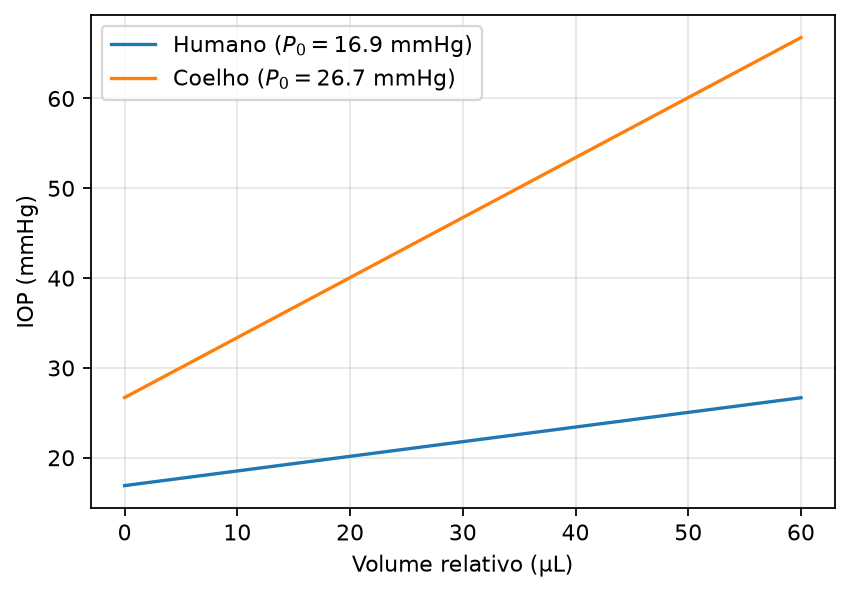
\includegraphics[width=0.55\textwidth]{Figuras/fig1_linear_comparativo.png}
\caption{Forma linear de $P(V)$, humano ($P_0=\SI{16{,}9}{\milli\meter Hg}$) e coelho anestesiado ($P_0=\SI{26{,}7}{\milli\meter Hg}$), cada um no seu próprio ponto de equilíbrio fisiológico (Seção~\ref{sec:producao_trabecular}). É a única forma usada para o coelho neste relatório, com o mesmo $E=\SI{3{,}0}{\mega\pascal}$ (estimativa de trabalho, Tabela~\ref{tab:E_esclera}). Para $\SI{50}{\micro\liter}$, o pico linear previsto para o coelho fica em torno de $\SI{60}{\milli\meter Hg}$, ordem de grandeza sem confronto clínico neste documento.}
\label{fig:linear_comparativo}
\end{figure}
 
A segunda forma é a lei de Friedenwald, que descreve o comportamento observado em olhos reais de maneira exponencial \citep{friedenwald1937},
 
\begin{equation}
\log_{10} P = \log_{10} P_0 + K_f\,(V-V_0),
\label{eq:friedenwald}
\end{equation}

onde $K_f$ é o coeficiente de rigidez ocular de Friedenwald e $V_0$ é o volume de referência no qual $P=P_0$ (neste relatório, $V_0=0$ no estado basal adotado antes da injeção). A curva $P(V)$ do globo reflete a parede corneoescleral \citep{ethier2004biomech}. Com $E=3{,}0$ MPa, a forma linear ($K=0{,}163$ mmHg/µL) fica $\approx24\%$ abaixo da curva de Friedenwald em 50 µL. Em olhos humanos vivos, o coeficiente foi medido por injeção manométrica direta de volume, com $K_f=0{,}0126\ \unit{\per\micro\liter}$ \citep{pallikaris2005}, e estimado por pneumotonometria diferencial, que não injeta volume, com $K_f=0{,}0252\ \unit{\per\micro\liter}$ em olhos normais \citep{kazemi2021}. Este último estudo também encontra rigidez menor em olhos com glaucoma ($K_f=0{,}0218\ \unit{\per\micro\liter}$).
 
Os valores de $K_f$ discutidos acima divergem, e a diferença de mecanismo e de faixa de medida é a explicação mais plausível, resumida na Tabela~\ref{tab:kf_comparacao}. 
 
\begin{table}[htbp]
\centering
\caption{Os três valores de $K_f$ usados ou discutidos neste relatório, com o mecanismo de medição e a particularidade que explica a divergência entre eles.}
\label{tab:kf_comparacao}
\small
\begin{tabular}{p{2.4cm}p{1.5cm}p{4.4cm}p{5.3cm}}
\toprule
Fonte & $K_f$ & O que mede & Particularidade \\
\midrule
\citet{pallikaris2005} &
$0{,}0126$ &
Injeção manométrica direta na câmara anterior, $79$ olhos de cirurgia de catarata, perturbação grande (até $200\ \unit{\micro\liter}$, em passos de $4{,}5\ \unit{\micro\liter}$) &
Mecanismo mais parecido com o deste relatório, mas calibrado só entre $10$ e $\SI{35}{\milli\meter Hg}$ de IOP, partindo de $\SI{10}{\milli\meter Hg}$. Extrapolar para picos acima de $\SI{50}{\milli\meter Hg}$ sai da faixa validada. \\
\addlinespace
\citet{kazemi2021} &
$0{,}0252$ normal\newline $0{,}0218$ glaucoma &
Pneumotonometria diferencial (IOP medida com e sem um peso de $10\ \unit{\gram}$ na ponteira, decúbito dorsal). Diferença de leitura convertida em $\Delta V$ equivalente por tabela de calibração, sem injeção real &
Perturbação mecânica externa minúscula, não injeção de volume. Mede rigidez de repouso, não resposta a bolus grande. Compara diretamente normal vs. glaucoma no mesmo protocolo. O intervalo de confiança de $95\%$ do grupo normal vai de $0{,}0230$ a $0{,}0280$. \\

\addlinespace
Recalibrado (este relatório) &
$0{,}00504$--$0{,}00656$\newline ($0{,}00581$ adotado) &
Não é medido. É a inversão algébrica da lei de Friedenwald usando o pico do \citet{knecht2009} como alvo, a partir do basal $P_0=\SI{16{,}9}{\milli\meter Hg}$ adotado neste relatório (Seção~\ref{sec:producao_trabecular}). Os limites vêm dos picos precisos relatados ($30{,}19$ e $35{,}97$ mmHg). O valor adotado vem do alvo $P=\SI{33}{\milli\meter Hg}$ (centro arredondado do intervalo $30$--$36$ relatado pelo estudo) &
Único calibrado exatamente no cenário de interesse (mesmo volume, mesma via, pico agudo real), mas por construção matemática, não por manometria, e depende de um único estudo. Trata-se de um $K_f$ efetivo de ajuste ($2$--$4\times$ abaixo dos $K_f$ manométricos ou pneumotonométricos acima), sensível ao basal assumido. Com $P_0=\SI{14}{\milli\meter Hg}$ e o mesmo pico-alvo, $K_f\approx0{,}00745$ ($+28\%$). Com $P_0=\SI{22}{\milli\meter Hg}$, $K_f\approx0{,}00352$ ($-39\%$). O Knecht não reporta basal único para a inversão. \\
\bottomrule
\end{tabular}
\end{table}
 
A Figura~\ref{fig:humano_pv} compara a forma linear de casca com três leis de Friedenwald para $P_0=\SI{16{,}9}{\milli\meter Hg}$, usando $K_f$ de \citet{pallikaris2005}, de \citet{kazemi2021} e a recalibração contra o pico de IVI de \citet{knecht2009} (Tabela~\ref{tab:kf_comparacao}). Só a recalibrada ($K_f=0{,}00581$ µL$^{-1}$) entra na dinâmica do WP0. Em $\SI{50}{\micro\liter}$ ela dá $\approx\SI{33}{\milli\meter Hg}$, a mais branda entre as candidatas. A linear prevê $\SI{25}{\milli\meter Hg}$ e fica abaixo do alvo de calibração. Com o $K_f$ de \citet{pallikaris2005} na forma $P=P_0\,10^{K_f V}$ (Equação~\ref{eq:friedenwald} em escala log), a projeção sobe para $\SI{72{,}1}{\milli\meter Hg}$. Se, em vez de multiplicar $P_0$, soma-se a ele o $\Delta P$ que \citet{pallikaris2005} mediu na câmara anterior a partir de $\SI{10}{\milli\meter Hg}$ ($P=P_0+\Delta P_{\text{art}}$), o pico cai para $\approx\SI{49{,}6}{\milli\meter Hg}$. A curva de \citet{kazemi2021} serve só de referência no painel e extrapola para valores não plausíveis em $\SI{50}{\micro\liter}$ (Seção~\ref{sec:camada2_pico}).
 
\begin{figure}[htbp]
\centering
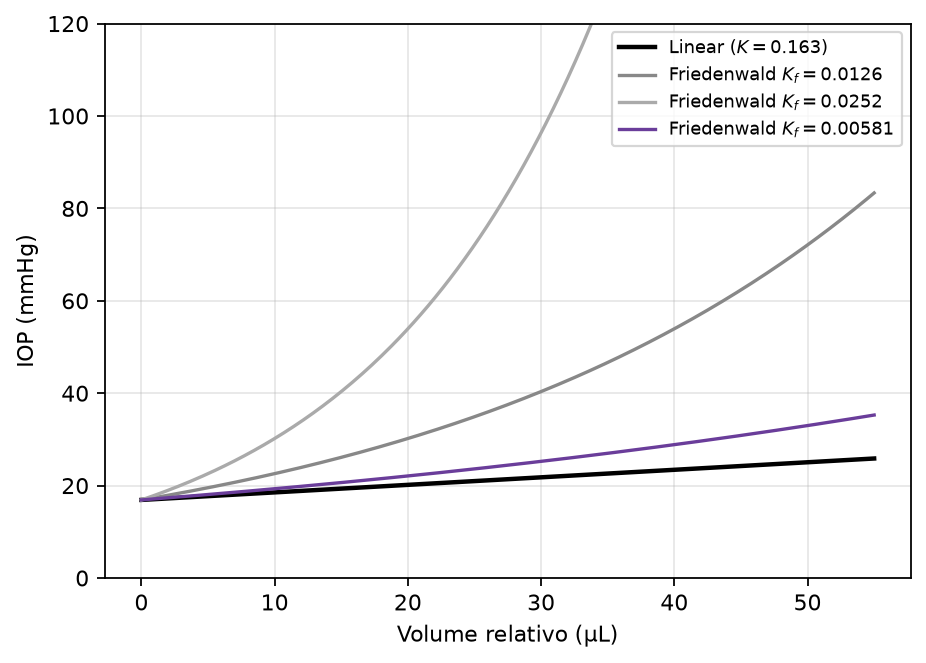
\includegraphics[width=0.62\textwidth]{Figuras/fig2_humano_friedenwald.png}
\caption{Forma linear e Friedenwald para humano com $P_0=\SI{16{,}9}{\milli\meter Hg}$. Curvas com $K_f$ de \citet{pallikaris2005}, \citet{kazemi2021} e recalibração contra o pico de \citet{knecht2009} ($K_f=\SI{0{,}00581}{\per\micro\liter}$, $\SI{33}{\milli\meter Hg}$ em $\SI{50}{\micro\liter}$). Em $\SI{50}{\micro\liter}$, \citet{pallikaris2005} dá $\SI{72{,}1}{\milli\meter Hg}$ com $P=P_0\,10^{K_f V}$ e $\approx\SI{49{,}6}{\milli\meter Hg}$ com $P=P_0+\Delta P_{\text{art}}$. \citet{kazemi2021} extrapola para $\SI{307{,}5}{\milli\meter Hg}$. Eixo cortado em $\SI{120}{\milli\meter Hg}$.}
\label{fig:humano_pv}
\end{figure}
 
\subsection{Injeção Intravítrea}
 
A injeção intravítrea é modelada como uma rampa de vazão constante durante um intervalo curto de tempo,
 
\begin{equation}
Q_{\text{ivi}}(t) =
\begin{cases}
\dfrac{V_{\text{inj}}}{\Delta t_{\text{inj}}}, & t_0 \le t \le t_0+\Delta t_{\text{inj}}, \\[6pt]
0, & \text{caso contrário},
\end{cases}
\label{eq:ivi}
\end{equation}
 
onde $V_{\text{inj}}$ é o volume total injetado e $\Delta t_{\text{inj}}$ é a duração da injeção. Adota-se $\Delta t_{\text{inj}}=\SI{6}{\second}$ (premissa do modelo). Essa é a única fonte de entrada de volume além da produção fisiológica, e é ela que provoca o pico agudo de pressão. O trabalho de \citet{ruffini2024} modela a expansão e a deflação do globo após a injeção com uma estrutura de balanço semelhante, mas sem detalhar a injeção como uma rampa de duração finita.
 
A justificativa para tratar essa etapa como quase estática, sem necessidade de resolver o escoamento do fluido dentro do olho, vem da comparação entre duas escalas de tempo. A velocidade com que uma variação de pressão se propaga através da parede elástica do globo é estimada pela relação de Moens e Korteweg \citep{fung1997},
 
\begin{equation}
c_{\text{MK}} = \sqrt{\frac{E\,t}{2\,\rho\,R}},
\label{eq:moens_korteweg}
\end{equation}
 
onde $\rho$ é a densidade do fluido. A fórmula completa de Korteweg inclui a compressibilidade do líquido, $c=\sqrt{(K_{\mathrm{B}}/\rho)\,/\,[1+K_{\mathrm{B}} D/(E t)]}$, em que $K_{\mathrm{B}}=\SI{2{,}2}{\giga\pascal}$ é o módulo de compressibilidade do líquido e $D$ o diâmetro. Aqui $K_{\mathrm{B}} D/(Et)\approx3{,}5\times10^{4}\gg1$, de modo que a parede complacente é o fator limitante da onda e a Equação~\ref{eq:moens_korteweg} é uma boa aproximação. A velocidade do som no líquido ($\approx\SI{1500}{\meter\per\second}$) só seria relevante com parede rígida. Usando $E=\SI{3{,}0}{\mega\pascal}$, com $t=\SI{0{,}5}{\milli\meter}$, $\rho=\SI{1000}{\kilo\gram\per\meter\cubed}$ e $R=\SI{12}{\milli\meter}$, o resultado é $c_{\text{MK}}\approx\SI{7{,}9}{\meter\per\second}$. Calculado para um diâmetro total do globo de $\SI{24}{\milli\meter}$, a onda atravessa o globo em $\approx\SI{3}{\milli\second}$, muito inferior a $\Delta t_{\text{inj}}$. Isso justifica que a parede acompanhe quase instantaneamente o bolus, assumindo um único compartimento pressurizado.
 
\subsection{Refluxo pelo trajeto da agulha}
 
Após a retirada da agulha, uma pequena quantidade de líquido pode escapar pelo canal deixado na esclera. Esse fenômeno é modelado não como uma vazão contínua, como a injeção, mas como uma perda de volume instantânea, aplicada no exato momento em que a injeção termina,
 
\begin{equation}
V(t_0+\Delta t_{\text{inj}}^+) = V(t_0+\Delta t_{\text{inj}}^-) - \Delta V_{\text{refluxo}}.
\label{eq:refluxo}
\end{equation}
 
Essa escolha de modelagem reflete uma observação experimental em olhos suínos \citep{brodie2014}, com refluxo em jato no instante da retirada da agulha, volume médio $\approx1{,}19$ µL, sem vazamento prolongado. O mesmo $\Delta V_{\text{refluxo}}$ é aplicado ao humano como ordem de grandeza. A composição do refluxo, majoritariamente vítreo \citep{brodie2014}, não entra no balanço, que depende só do volume que deixa a cavidade.
 
No presente estudo, com $P_0=\SI{16{,}9}{\milli\meter Hg}$, na forma linear ($K=0{,}163$), o pico de $\SI{25{,}0}{\milli\meter Hg}$ cai para $\SI{24{,}8}{\milli\meter Hg}$ logo após o refluxo, uma queda de $\SI{0{,}19}{\milli\meter Hg}$. Na forma Friedenwald recalibrada ($K_f=0{,}00581$, pico de $\SI{32{,}9}{\milli\meter Hg}$), a queda é de $\SI{0{,}52}{\milli\meter Hg}$ (de $32{,}90$ para $\SI{32{,}38}{\milli\meter Hg}$), $2{,}7$ vezes maior em valor absoluto. Ambas disponíveis na Figura~\ref{fig:refluxo_humano}.

Mesmo o maior dos dois valores ($0{,}52\ \unit{\milli\meter Hg}$, Friedenwald recalibrada) está abaixo da resolução prática da tonometria de aplanação de Goldmann, em geral lida em incrementos de $\SI{1}{\milli\meter Hg}$ \citep{goldmannschmidt1957}.

\FloatBarrier
\begin{figure}[htbp]
\centering
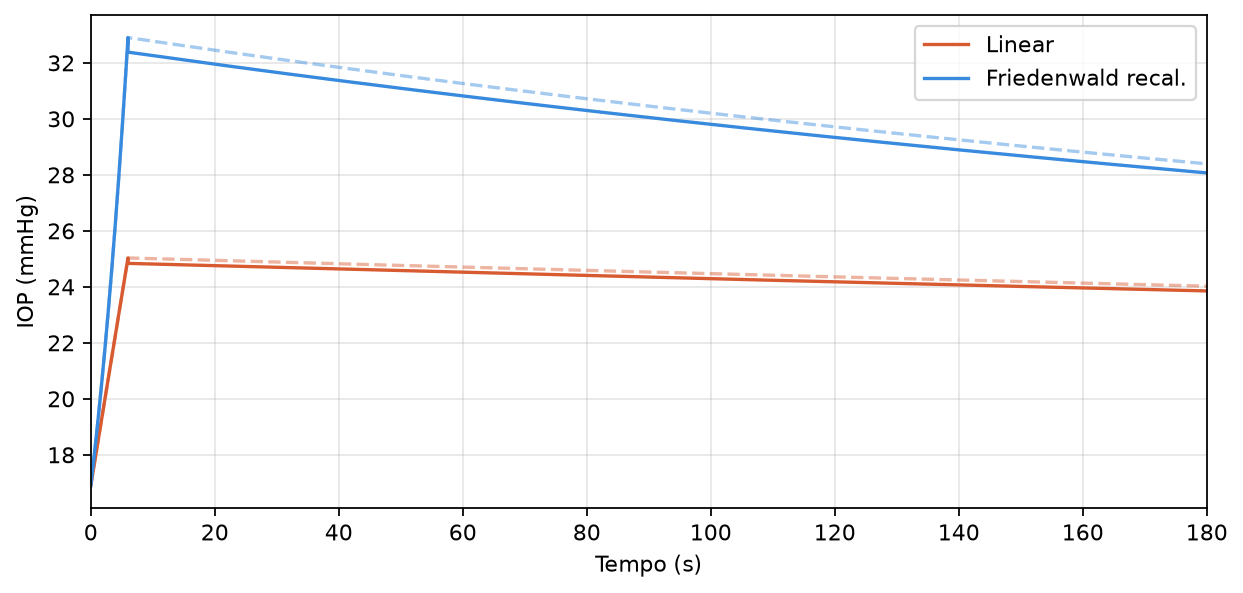
\includegraphics[width=0.95\textwidth]{Figuras/fig_refluxo_humano.png}
\caption{Efeito do refluxo sobre a curva de IOP, humano ($P_0=\SI{16{,}9}{\milli\meter Hg}$), zoom nos primeiros $3$ minutos, linear e Friedenwald recalibrada (linha contínua com refluxo, tracejada sem refluxo). A queda logo após o refluxo é maior em Friedenwald porque a lei exponencial amplifica a queda proporcionalmente ao próprio valor da pressão. Nas duas formas, as curvas convergem novamente ao longo do decaimento, porque o refluxo desloca o ponto de partida, não a dinâmica de retorno ao basal.}
\label{fig:refluxo_humano}
\end{figure}

\subsection{Paracentese}
 
A paracentese é modelada como um escoamento governado pela lei de Poiseuille através de uma agulha, durante um intervalo de tempo,
 
\begin{equation}
Q_{\text{par}}(t,P) =
\begin{cases}
\dfrac{(P-P_{\text{atm}})}{R_{\text{par}}}, & t_{\text{par}} \le t \le t_{\text{par}}+\Delta t_{\text{par}}, \\[6pt]
0, & \text{caso contrário},
\end{cases}
\label{eq:par_vazao}
\end{equation}
 
onde $R_{\text{par}}$ é a resistência hidráulica do trajeto de drenagem, calculada a partir do raio interno e do comprimento da agulha utilizada \citep{white2011},
 
\begin{equation}
R_{\text{par}} = \frac{8\,\mu\,L}{\pi\,a^4}
\label{eq:par_resistencia}
\end{equation}
 
em que $\mu$ é a viscosidade do humor aquoso, $L$ é o comprimento do trajeto percorrido pelo fluido e $a$ é o raio interno \citep{white2011}. Diferentemente do refluxo, a paracentese é tratada como um processo contínuo dentro da sua janela de atuação, pois o instrumento permanece inserido durante a drenagem, e o fluido efetivamente percorre todo o comprimento do seu canal interno.

Os parâmetros usados na Equação~\ref{eq:par_resistencia} incluem raio interno $a=\SI{0{,}0795}{\milli\meter}$ (diâmetro interno $\SI{0{,}159}{\milli\meter}$, agulha calibre $30$G) \citep{henein2019}, comprimento do trajeto $L=\SI{13}{\milli\meter}$ \citep{aiello2004, doshi2011, henein2019} e viscosidade do humor aquoso $\mu=\SI{0{,}75}{\milli\pascal\second}$ (próxima à da água a $\SI{37}{\celsius}$) \citep{heys2001, dvoriashyna2019, repetto2015}, resultando em $R_{\text{par}}=6{,}2\times10^{11}\ \unit{\pascal\second\per\meter\cubed}$ segundo a lei de Hagen--Poiseuille \citep{ocularfluiddynamics, peng2025}.
 
A duração da janela, $\Delta t_{\text{par}}$, não possui registro na literatura e, por isso, é calculada como o tempo necessário para drenar o volume retirado, adotado igual ao volume injetado, $\SI{50}{\micro\liter}$ \citep{changchung2007, soheilian2017}, e a paracentese é encerrada quando esse volume é atingido. Esse tempo não é uma constante da agulha, porque depende da pressão em que a drenagem começa. Como a vazão é proporcional à pressão, e a pressão diminui à medida que o volume escoa, a drenagem desacelera ao longo do processo.
 
Integrando numericamente a Equação~\ref{eq:par_vazao} para a retirada de $\SI{50}{\micro\liter}$, o resultado depende do ponto de partida. A partir da pressão basal ($\SI{16{,}9}{\milli\meter Hg}$), a drenagem leva $\Delta t_{\text{par}}=\SI{18{,}8}{\second}$ na forma linear e $\SI{19{,}6}{\second}$ na recalibrada. A partir da pressão já elevada pela injeção, leva de $\SI{10{,}5}{\second}$ a $\SI{11{,}8}{\second}$, porque a vazão inicial é maior. Como verificação de ordem de grandeza, mesmo que a pressão permanecesse em $\SI{16{,}9}{\milli\meter Hg}$ durante toda a drenagem, a vazão inicial de $\SI{3{,}6}{\micro\liter\per\second}$ exigiria $\SI{13{,}8}{\second}$, de modo que nenhuma duração inferior a esse valor é compatível com a retirada de $\SI{50}{\micro\liter}$ a partir do basal. 

O escoamento na agulha é laminar e desenvolvido, com $Q\approx\SI{3{,}6}{\micro\liter\per\second}$, o número de Reynolds é $\approx39$ e o comprimento de entrada ($\approx0{,}06\,Re\,d$) é $\approx\SI{0{,}4}{\milli\meter}$, pequeno frente a $L=\SI{13}{\milli\meter}$, o que valida a lei de Poiseuille.
 
Este relatório simula três instantes distintos de início da paracentese em relação à injeção, correspondendo a três estratégias clínicas diferentes, descritas a seguir.
 
\begin{itemize}
\item Profilática ($t=-\SI{30}{\second}$ antes da injeção): realizada de $t=-\SI{30}{\second}$ até $t=-\SI{11{,}2}{\second}$ na forma linear ($\Delta t_{\text{par}}=\SI{18{,}8}{\second}$) ou até $t=-\SI{10{,}4}{\second}$ na recalibrada ($\Delta t_{\text{par}}=\SI{19{,}6}{\second}$), terminando, portanto, entre $\SI{10{,}4}{\second}$ e $\SI{11{,}2}{\second}$ antes do início da injeção. É o desenho usado por protocolos como o de \citet{soheilian2017}, e é modelada aqui como três fases sequenciais e não sobrepostas (paracentese, intervalo livre residual, depois injeção).
\item Reativa ($t=+\SI{30}{\second}$ após a injeção): realizada assim que se percebe uma elevação de pressão, mas o pico agudo, que se forma em segundos, já ocorreu. A drenagem começa em pressão elevada e leva $\SI{11{,}5}{\second}$ na forma linear e $\SI{10{,}5}{\second}$ na recalibrada.
\item Tardia ($t=+\SI{2}{\minute}$ após a injeção): realizada bem depois que o pico já se formou por completo, seguindo prática relatada por oftalmologistas que preferem confirmar a elevação antes de intervir. A drenagem leva $\SI{11{,}8}{\second}$ na forma linear e $\SI{11{,}3}{\second}$ na recalibrada.
\end{itemize}
 
Como a paracentese profilática termina antes de a injeção começar e o pico se forma durante $\Delta t_{\text{inj}}$, apenas a profilática consegue reduzir o próprio pico. A reativa e a tardia começam depois que o pico já aconteceu.
 
De acordo com os resultados obtidos por \citet{soheilian2017}, um grupo sem paracentese, com IOP basal de $14{,}2\pm2{,}0\ \unit{\milli\meter Hg}$, sobe para $40{,}6\ \unit{\milli\meter Hg}$ aos dois minutos (aumento de $+26{,}4\pm5{,}7$), caindo para $20{,}7\ \unit{\milli\meter Hg}$ aos trinta minutos. Um grupo com paracentese profilática, com IOP basal de $13{,}8\pm2{,}3\ \unit{\milli\meter Hg}$, vai para apenas $12{,}5\ \unit{\milli\meter Hg}$ aos dois minutos (variação de $-1{,}3\pm2{,}4$) e $10{,}6\ \unit{\milli\meter Hg}$ aos trinta minutos (variação de $-3{,}2\pm1{,}8$).
 
A Figura~\ref{fig:paracentese_humano} mostra que, na forma recalibrada, o pico cai de $\SI{32{,}9}{\milli\meter Hg}$ (sem intervenção) para $\SI{17{,}1}{\milli\meter Hg}$ na profilática, uma redução de $48\%$. Na forma linear, o pico cai de $\SI{25{,}0}{\milli\meter Hg}$ para $\SI{17{,}1}{\milli\meter Hg}$, uma redução de $32\%$, menor em valor absoluto porque o pico linear já é pequeno mesmo sem intervenção. Como o volume retirado é igual ao injetado, a profilática anula o efeito da injeção, a drenagem leva a pressão a $\SI{8{,}7}{\milli\meter Hg}$ na forma recalibrada e a $\SI{8{,}8}{\milli\meter Hg}$ na linear, e a injeção a traz de volta ao redor do basal, sem ultrapassá-lo. Reativa e tardia não alteram o pico. Na forma recalibrada, a pressão mínima é $\SI{16{,}2}{\milli\meter Hg}$ (reativa, $+30$ s) e $\SI{15{,}0}{\milli\meter Hg}$ (tardia, $+2$ min), mais baixa quanto mais tarde a intervenção, porque, quanto mais tempo passa, mais do volume injetado já saiu pelas vias fisiológicas, e a retirada de $\SI{50}{\micro\liter}$ passa a ultrapassar o excesso. Nas estratégias reativa e tardia, o retorno final ao basal ocorre por produção fisiológica, muito mais lento do que a queda induzida pela paracentese em si.
 
\begin{figure}[htbp]
\centering
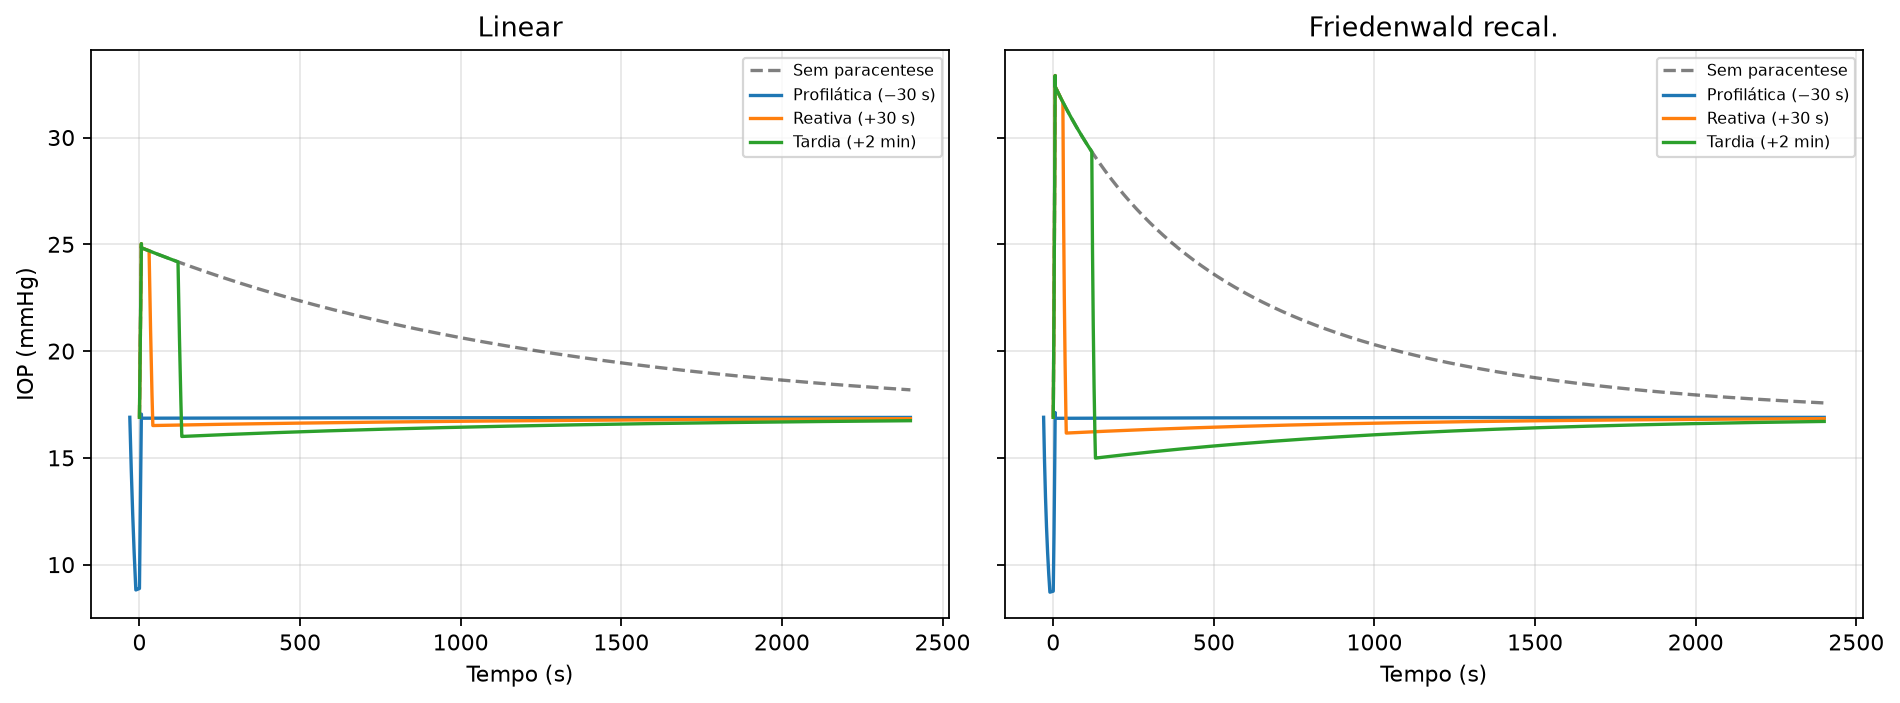
\includegraphics[width=0.98\textwidth]{Figuras/fig_paracentese_3cenarios.png}
\caption{Efeito da paracentese sobre a curva de IOP em três estratégias (linhas: profilática $t=-30$s, reativa $t=+30$s, tardia $t=+2$min), com a drenagem encerrada ao atingir $\SI{50}{\micro\liter}$, contra as duas formas de $P(V)$ efetivamente usadas neste relatório.}
\label{fig:paracentese_humano}
\end{figure}
 
\subsection{Produção trabecular e uveoescleral}
\label{sec:producao_trabecular}
 
O escoamento do humor aquoso, responsável por trazer a pressão de volta ao valor basal após a injeção, ocorre por duas vias distintas. A via trabecular é a via convencional descrita pela relação de Goldmann \citep{goel2010,brubaker2004},
 
\begin{equation}
Q_{TM}(P) = C_{\text{out}}\,(P-P_{ev}),
\label{eq:trabecular}
\end{equation}
 
onde $C_{\text{out}}$ é a facilidade de escoamento trabecular e $P_{ev}$ é a pressão venosa episcleral. Na implementação numérica, $Q_{TM}$ não é truncado em zero quando $P<P_{ev}$. Na paracentese profilática, a forma recalibrada atinge $\approx\SI{8{,}7}{\milli\meter Hg}<P_{ev}=\SI{10}{\milli\meter Hg}$. O influxo trabecular resultante é de $\approx\SI{0{,}36}{\micro\liter\per\minute}$ e altera a IOP em menos de $\SI{0{,}02}{\milli\meter Hg}$.
 
A via uveoescleral, por sua vez, drena uma parte do humor aquoso de maneira quase independente da IOP, sendo descrita apenas como uma fração da produção total,
 
\begin{equation}
Q_{uv} = f_{uv}\,Q_{\text{prod}}.
\label{eq:uveoscleral}
\end{equation}
 
A fração $f_{uv}$ varia entre espécies, sendo pequena em coelhos e gatos, devido ao pouco desenvolvimento do músculo ciliar nessas espécies, e substancialmente maior em primatas e humanos \citep{alm2009}. A Tabela~\ref{tab:especies} reúne os valores experimentais disponíveis nas espécies discutidas neste relatório.
 
\begin{table}[htbp]
\centering
\caption{Parâmetros de escoamento fisiológico por espécie, com fonte.}
\label{tab:especies}
\begin{tabular}{lp{4.2cm}p{4.2cm}}
\toprule
 & \centering Humano & \centering\arraybackslash Coelho (anestesiado) \\
\midrule
$Q_{\text{prod}}$ (\unit{\micro\liter\per\minute}) & $2{,}4\pm0{,}6$ \citep{goel2010} & $3{,}06\pm0{,}6$ \citep{kiel2011ciliary} \\
$C_{\text{out}}$ (\unit{\micro\liter\per\minute\per\milli\meter Hg}) & $0{,}28$ \citep{goel2010} & $0{,}26\pm0{,}07$ \citep{fourman1989outflow} \\
$P_{ev}$ (\unit{\milli\meter Hg}) & $10$ \citep{ethier2004biomech} & $15$--$16$ \citep{kiel2015evp} \\
$f_{uv}$ (\% do total) & $\approx 20$ \citep{goel2010,alm2009} & $3$--$8$ \citep{alm2009} \\
\bottomrule
\end{tabular}
\end{table}
 
Fixa-se $P_0=\SI{16{,}9}{\milli\meter Hg}$. Com $Q_{\text{prod}}=\SI{2{,}4}{\micro\liter\per\minute}$ e os demais valores da Tabela~\ref{tab:especies}, o repouso seria $\SI{16{,}86}{\milli\meter Hg}$. Para fechar $\SI{16{,}9}{\milli\meter Hg}$ com $dV/dt=0$ sem injeção, adota-se $Q_{\text{prod}}=\SI{2{,}415}{\micro\liter\per\minute}$, dentro de $2{,}4\pm0{,}6$. O basal vem do equilíbrio $P_0=P_{ev}+Q_{\text{prod}}(1-f_{uv})/C_{\text{out}}$.
 
Aplicando o mesmo cálculo aos parâmetros do coelho anestesiado ($Q_{\text{prod}}=3{,}06$, $C_{\text{out}}=0{,}26$, $f_{uv}=0{,}05$, $P_{ev}=15{,}5$, meio da faixa $15$--$16$), o resultado é $P_0=15{,}5+3{,}06\times0{,}95/0{,}26\approx\SI{26{,}7}{\milli\meter Hg}$. Esse valor é consistente com a IOP basal de coelho anestesiado relatada entre $16{,}2$ e $\SI{33{,}2}{\milli\meter Hg}$ \citep{kiel2015evp}, contra apenas $7$--$\SI{16}{\milli\meter Hg}$ em coelho acordado. O valor de $C_{\text{out}}$ usado, medido em coelho não anestesiado, é o único disponível na literatura revisada. Não foi encontrada uma medição direta de $C_{\text{out}}$ sob anestesia geral.
 
Os dois termos do escoamento, trabecular e uveoescleral, são responsáveis pela recuperação do equilíbrio após o término da injeção. O quão rápido isso acontece está associado à constante de tempo
 
\begin{equation}
\tau = \frac{1}{C_{\text{out}}\,K},
\label{eq:tau}
\end{equation}
 
que resulta da linearização da equação de balanço em torno do estado de equilíbrio, e que determina o perfil de resposta do sistema. Para o coelho, que usa a forma linear, $K$ nessa fórmula é a mesma constante $K=0{,}668$ da Equação~\ref{eq:casca_fina}. Para o humano recalibrado, usa-se $K_{\text{local}}=dP/dV$ no basal, $K_{\text{local}}=\ln(10)\cdot K_f\cdot P_0=2{,}30\times0{,}00581\times16{,}9\approx\SI{0{,}226}{\milli\meter Hg\per\micro\liter}$, o que com $C_{\text{out}}=0{,}28$ dá $\tau=1/(0{,}28\times0{,}226)\approx\SI{15{,}8}{\minute}$.

A Figura~\ref{fig:decaimento} mostra a curva completa de retorno ao valor basal, para humano e coelho, com a constante de tempo de cada espécie ($\tau_{\text{humano}}=\SI{15{,}8}{\minute}$ no basal, $\tau_{\text{coelho}}=\SI{5{,}76}{\minute}$). No humano, a rigidez local da forma de Friedenwald cresce com a pressão, de modo que $\tau$ cai para $\SI{8{,}1}{\minute}$ no pico e a queda é mais rápida no início, aproximando-se de $\SI{15{,}8}{\minute}$ ao final. Com refluxo ligado, aos $10$ min dissipa-se cerca de $64\%$ do excesso pós-pico, aos $50$ min, $98\%$.
 
\begin{figure}[htbp]
\centering
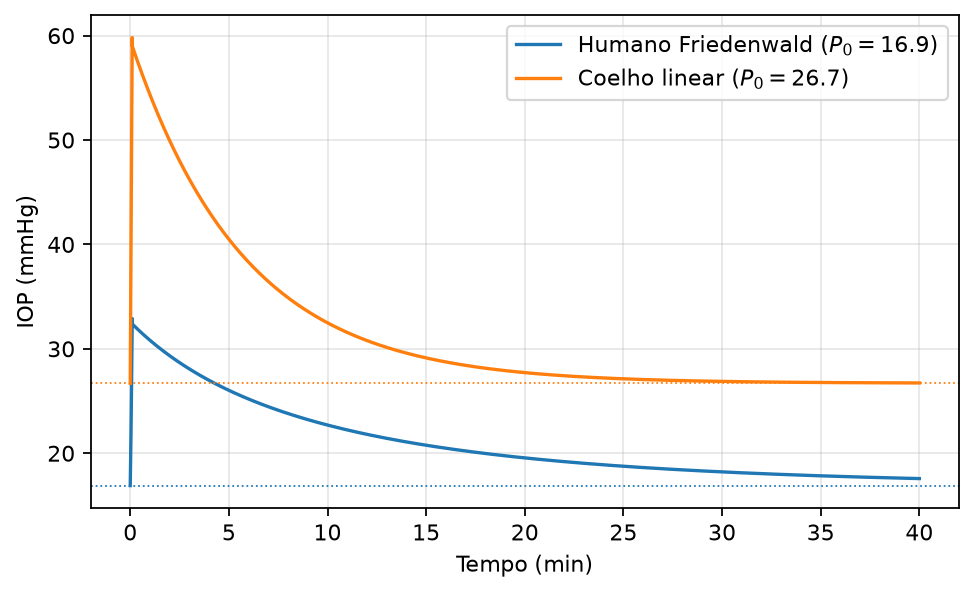
\includegraphics[width=0.65\textwidth]{Figuras/fig_decaimento.png}
\caption{Retorno ao basal após injeção de $\SI{50}{\micro\liter}$ via escoamento trabecular e uveoescleral combinados, humano ($P_0=\SI{16{,}9}{\milli\meter Hg}$) e coelho anestesiado ($P_0=\SI{26{,}7}{\milli\meter Hg}$). No basal, o $\tau$ do coelho ($\SI{5{,}76}{\minute}$) é $2{,}7$ vezes menor que o do humano ($\SI{15{,}8}{\minute}$).}
\label{fig:decaimento}
\end{figure}
 
\section{Verificação}
\label{sec:validacao}
 
\subsection{Parte 1 --- verificação numérica}
\label{sec:camada1_ruffini}

Antes de qualquer comparação com dado biológico, verifica-se se o solver resolve corretamente a equação diferencial. Para isso, utiliza-se o artigo de \citet{ruffini2024}, que também descreve um modelo 0D linear, com produção efetiva de $Q_{in}=2{,}2\ \unit{\micro\liter\per\minute}$, pressão episcleral de $P_{ev}=\SI{8}{\milli\meter Hg}$ e complacência ocular constante de $C=\SI{1}{\micro\liter\per\milli\meter Hg}$ (rigidez $K\approx0{,}05\ \unit{\per\micro\liter}$ medida por \citet{collins1980mathematical} na base natural, $\ln P=\ln P_0+K(V-V_0)$, equivalente a $K_f\approx0{,}05/\ln(10)\approx0{,}022\ \unit{\per\micro\liter}$ na forma em $\log_{10}$ da Equação~\ref{eq:friedenwald}), obtendo analiticamente uma constante de tempo de decaimento $\tau=\SI{3{,}18}{\minute}$ (valor arredondado do resumo). No protocolo de verificação deste relatório ($\SI{50}{\micro\liter}$ em $\SI{6}{\second}$, refluxo desligado, $f_{uv}=0$, $C_{\text{out}}=Q_{in}/(P_{\text{eq}}-P_{ev})$ com $P_{\text{eq}}=\SI{15}{\milli\meter Hg}$ de equilíbrio do teste), o valor analítico linearizado é $\tau_{\text{analítico}}=1/(C_{\text{out}}K)=\SI{3{,}18}{\minute}$. Um ajuste exponencial da curva simulada (baseline fixa em $\SI{15}{\milli\meter Hg}$, janela a partir do fim da injeção) reproduz esse $\tau$ com erro relativo de $\approx3{,}9\times10^{-7}$ (inferior a $10^{-6}$).
 
\subsection{Parte 2 --- pico agudo}
\label{sec:camada2_pico}
 
A Tabela~\ref{tab:literatura_master} reúne todas as fontes de literatura usadas neste relatório para calibrar ou validar a resposta de pressão pós-IVI, com espécie, volume de injeção, basal, pico e tipo de intervenção.
 
\begin{table}[htbp]
\centering
\caption{Fontes de literatura usadas na parametrização e validação deste relatório (todas em humanos).}
\label{tab:literatura_master}
\small
\resizebox{\textwidth}{!}{
\setlength{\tabcolsep}{5pt}
\begin{tabular}{p{2.4cm}p{1.9cm}p{1.7cm}p{1.7cm}p{6.5cm}}
\toprule
Fonte & IVI & Basal (mmHg) & Pico (mmHg) & Paracentese \\
\midrule
\citet{knecht2009} & $50$\,µL & --- & $30{,}2$--$36{,}0$ & Alvo de calibração de $K_f=0{,}00581$ (recalibrado) \\
\citet{soheilian2017}, Grupo A & $50$\,µL & $14{,}2$ & $40{,}6$ & Sem intervenção \\
\citet{soheilian2017}, Grupo B & $50$\,µL & $13{,}8$ & $12{,}5$ & Paracentese profilática \\
\citet{sharei2010} & $50$\,µL & $22{,}4$ & $47{,}9$ & Sem intervenção \\
\citet{hu2022conbercept} & $50$\,µL & $14{,}81$ & $26{,}80$ & Sem intervenção \\
\citet{papazoglou2026} & $50$\,µL & $13{,}98$ & $31{,}15$ (T2) & Sem intervenção \\
\citet{changchung2007} & $100$\,µL & $15{,}33$ & $46{,}7$ & Paracentese reativa/tardia (pós-paracentese $7{,}80$ mmHg). Volume diferente do padrão deste relatório \\
\bottomrule
\end{tabular}
}
 
\vspace{4pt}
\end{table}
\FloatBarrier
 
Nenhuma dessas fontes clínicas deriva ou mede $K_f$ diretamente. Os valores de $K_f$ usados neste relatório vêm exclusivamente da recalibração contra o Knecht (Seção~\ref{sec:balanco_geral}). As fontes clínicas de pico servem apenas para comparação externa do resultado final, não para parametrizar o modelo.

A Figura~\ref{fig:camada2} mostra as duas formas de $P(V)$ efetivamente usadas neste relatório junto com os pontos de pico medidos nos estudos sem intervenção.

\begin{figure}[htbp]
\centering
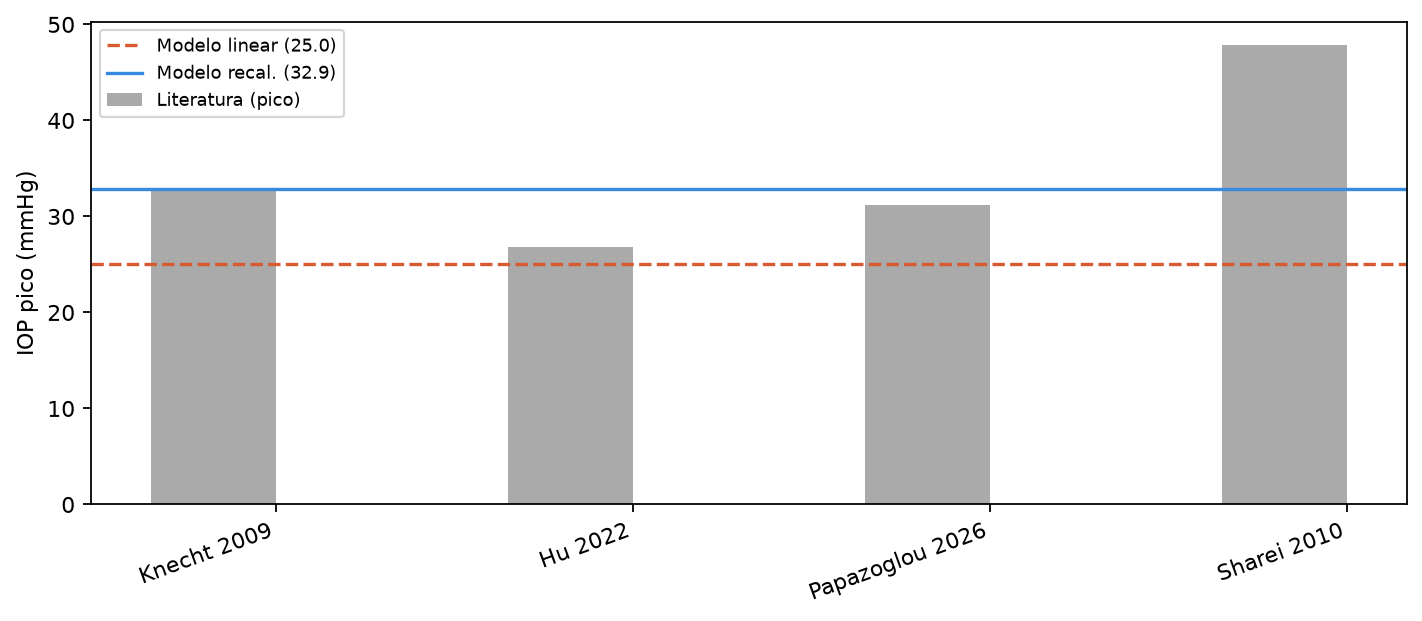
\includegraphics[width=0.85\textwidth]{Figuras/fig_camada2_picos.png}
\caption{Pico agudo pós-IVI para $\SI{50}{\micro\liter}$: as duas formas de $P(V)$ usadas neste relatório (sem paracentese, picos de $25{,}0$ e $\SI{32{,}9}{\milli\meter Hg}$ para linear e recalibrada, a partir de $P_0=\SI{16{,}9}{\milli\meter Hg}$) contra quatro estudos clínicos independentes (painel esquerdo: IOP absoluta; painel direito: aumento em relação ao basal de cada estudo). Os pontos clínicos correspondem a instantes de leitura diferentes (Tabela~\ref{tab:camada2_alinhada}).}
\label{fig:camada2}
\end{figure}
 
\citet{soheilian2017} relata, no grupo sem paracentese ($n=45$, bevacizumabe), IOP basal de $14{,}2\pm2{,}0\ \unit{\milli\meter Hg}$, subindo a $40{,}6\ \unit{\milli\meter Hg}$ aos dois minutos e caindo a $20{,}7\ \unit{\milli\meter Hg}$ aos trinta minutos.
 
\citet{sharei2010} relata, em $45$ olhos com ranibizumabe em posição supina, IOP basal de $22{,}4\pm5{,}5\ \unit{\milli\meter Hg}$ subindo a $47{,}9\pm15{,}1\ \unit{\milli\meter Hg}$ imediatamente após a injeção, com queda espontânea de $12{,}6$ aos três minutos e de $21$ aos dez minutos (pressões remanescentes $\approx35{,}3$ e $\approx26{,}9$ mmHg). O basal já elevado, característico da posição supina, explica o pico mais alto entre os estudos reunidos aqui.
 
\citet{hu2022conbercept} relata, em $40$ pacientes com Conbercept, IOP basal de $14{,}81\pm3{,}13\ \unit{\milli\meter Hg}$, subindo a $26{,}80\pm9{,}43\ \unit{\milli\meter Hg}$ aos dois minutos, $18{,}76\pm6{,}16$ aos dez minutos e $16{,}54\pm5{,}94$ aos trinta minutos.
 
\citet{papazoglou2026} mede IOP em três instantes. T1 é basal ($13{,}98\pm3{,}09\ \unit{\milli\meter Hg}$). T2 fica em $31{,}15\pm9{,}65\ \unit{\milli\meter Hg}$, com aquisição tipicamente iniciada em mediana $\approx\SI{7{,}5}{\minute}$ após a IVI. T3 fica dez minutos após T2 ($16{,}30\pm4{,}60\ \unit{\milli\meter Hg}$). Não é leitura imediata ao fim da agulha nem cota padronizada aos $2$ min.
 
\citet{knecht2009} relata pico medido em menos de um minuto de $35{,}97\pm8{,}13\ \unit{\milli\meter Hg}$ na técnica tunelizada e $30{,}19\pm12{,}14\ \unit{\milli\meter Hg}$ na técnica reta, mais convencional.

Os basais dos estudos diferem ($13{,}8$ a $\SI{22{,}4}{\milli\meter Hg}$), de modo que a comparação exige alinhar o instante de leitura. A Tabela~\ref{tab:camada2_alinhada} confronta, nesse instante, o aumento observado com o do modelo de referência (Friedenwald recalibrada, refluxo ligado, $P_0=\SI{16{,}9}{\milli\meter Hg}$).

\begin{table}[htbp]
\centering
\caption{Comparação alinhada no tempo: aumento de IOP ($\Delta P$) observado vs.\ modelo de referência.}
\label{tab:camada2_alinhada}
\small
\begin{tabular}{llrrr}
\toprule
Estudo & Instante & Observado & Modelo & Razão \\
\midrule
\citet{sharei2010} & imediato ($6$ s) & $+25{,}5$ & $+16{,}0$ & $1{,}6$ \\
\citet{soheilian2017} & $2$ min & $+26{,}4$ & $+12{,}4$ & $2{,}1$ \\
\citet{hu2022conbercept} & $2$ min & $+12{,}0$ & $+12{,}4$ & $1{,}0$ \\
\citet{papazoglou2026}, T2 & $\approx7{,}5$ min & $+17{,}2$ & $+7{,}2$ & $2{,}4$ \\
\bottomrule
\end{tabular}
\end{table}

O modelo subestima três dos quatro estudos em $1{,}6$ a $2{,}4\times$ e só concorda com \citet{hu2022conbercept}. Esse estudo reporta o menor aumento da Tabela~\ref{tab:camada2_alinhada} ($+12{,}0$ mmHg), de modo que a concordância pode ser coincidência com o extremo inferior da faixa clínica, e não acerto nos picos mais altos. O modelo reproduz, na prática, o limite inferior observado e subestima os demais. A forma linear ($K=0{,}163$ mmHg/µL) prevê, nos mesmos instantes, $+8{,}1$ mmHg ($6$ s) e $+7{,}3$ mmHg ($2$ min), ainda mais abaixo dos observados.

\subsection{Velocidade de retorno}
 
A terceira etapa testa não o pico, mas a velocidade com que a pressão volta ao normal depois dele. Para isso, \citet{lobue2023} mediram a IOP de $617$ pacientes a cada $10$ minutos após injeções de $\SI{0{,}05}{\milli\liter}$ e consideraram que o paciente havia retornado ao basal quando a IOP ficava a menos de $\SI{4}{\milli\meter Hg}$ do seu próprio valor pré-injeção. Isso ocorreu em $85\%$ dos pacientes aos $30$ minutos e em $98\%$ aos $50$ minutos. Na forma recalibrada, o olho do modelo atinge esse critério em $\SI{14{,}6}{\minute}$, antes dos $30$ minutos do percentil de $85\%$. O aumento médio observado aos $10$ minutos foi de $9\pm10$ mmHg e o modelo prevê $\SI{5{,}8}{\milli\meter Hg}$.
 
\subsection{Efeito da paracentese}
\label{sec:camada4}

Compara-se o efeito da paracentese contra três fontes da literatura. As três medem esse efeito da mesma forma, como a diferença de IOP entre um grupo com paracentese e um grupo sem, no mesmo instante.
 
\citet{soheilian2017} é a comparação mais direta, porque usa exatamente o volume de injeção deste relatório e divide a pesquisa em dois grupos, sem paracentese (Grupo A, pico de $40{,}6\ \unit{\milli\meter Hg}$ aos dois minutos) e com paracentese profilática (Grupo B, $12{,}5\ \unit{\milli\meter Hg}$ no mesmo instante). A diferença real entre os grupos é de $-28{,}1\ \unit{\milli\meter Hg}$ aos dois minutos e $-10{,}1\ \unit{\milli\meter Hg}$ aos trinta minutos. O cenário profilático simulado dá uma diferença de apenas $\SI{-12{,}5}{\milli\meter Hg}$ aos dois minutos e $\SI{-1{,}3}{\milli\meter Hg}$ aos trinta minutos. O modelo atual captura a direção do efeito, mas subestima a magnitude em ambos os instantes, por um fator de $2{,}3$ a $7{,}8\times$.

\citet{changchung2007} usa injeção de $\SI{100}{\micro\liter}$, o dobro do padrão deste relatório, o que impede comparar magnitudes de pico ou diferença aos dois minutos ($-38{,}9$ mmHg observados). Reporta-se apenas o contraste entre grupos aos quinze minutos, diferença real $-4{,}4$ mmHg contra $-4{,}8$ mmHg no cenário tardio simulado ($t_{\text{par}}=\SI{2}{\minute}$), ordem de grandeza semelhante.
 
\citet{zaman2025} agrega $13$ estudos clínicos com volumes e técnicas variadas, relatando diferenças médias de $-5{,}09\ \unit{\milli\meter Hg}$ aos dois minutos, $-2{,}37$ aos cinco minutos e $-1{,}54$ aos trinta minutos. Contra o mesmo cenário tardio simulado, o modelo dá $\SI{0{,}00}{\milli\meter Hg}$ aos dois minutos, $\SI{-10{,}8}{\milli\meter Hg}$ aos cinco minutos e $\SI{-1{,}7}{\milli\meter Hg}$ aos trinta minutos. O ajuste aos trinta minutos é bom ($-1{,}7$ contra $-1{,}5$), mas aos cinco minutos o modelo superestima o efeito em mais de $4\times$ ($-10{,}8$ contra $-2{,}4$).

Os três casos não mostram o mesmo padrão. Em \citet{soheilian2017}, com protocolo único e volume igual ao do modelo, o modelo subestima o efeito aos dois minutos, em boa parte porque a IOP prevista aos dois minutos sem intervenção ($\SI{29{,}3}{\milli\meter Hg}$) é menor que a observada no grupo A ($\SI{40{,}6}{\milli\meter Hg}$), embora o pico imediato simulado na forma recalibrada seja $\SI{32{,}9}{\milli\meter Hg}$. Esse desvio não se corrige variando $K_f$. Com o basal do próprio estudo ($14{,}2$ mmHg) e sem refluxo, a IOP simulada aos $2$ min vai de $\approx21$ a $\approx38$ mmHg quando $K_f$ sobe de $0{,}0035$ a $0{,}0150$ µL$^{-1}$ (pico imediato de $\approx21$ a $\approx78$ mmHg) e satura abaixo dos $40{,}6$ mmHg observados. Na faixa que cobre a incerteza do basal ($0{,}0035$ a $0{,}0075$), com $P_0=16{,}9$ mmHg, a IOP aos $2$ min chega a $\approx33{,}4$ mmHg e o pico imediato a $\approx40$ mmHg. Aos trinta minutos, o grupo B permanece abaixo do próprio basal ($-3{,}2$ mmHg), enquanto a profilática simulada já voltou ao basal.

Em \citet{changchung2007}, a diferença de $\SI{0{,}00}{\milli\meter Hg}$ aos dois minutos decorre do instante de início da paracentese simulada. Aos quinze minutos o modelo concorda com o observado ($-4{,}8$ contra $-4{,}4$).

Em \citet{zaman2025}, o modelo concorda aos trinta minutos ($-1{,}7$ contra $-1{,}5$) e superestima o efeito aos cinco ($-10{,}8$ contra $-2{,}4$). A paracentese simulada é um evento único e completo em $\SI{10{,}5}{\second}$ a $\SI{11{,}8}{\second}$, com queda abrupta logo depois. Quando o transitório já se dissipou, o que resta é dominado pela produção fisiológica.

\subsection{Limitações}
\label{sec:wp0_limitacoes}

Em comparação externa de pico (Seção~\ref{sec:camada2_pico}), o modelo subestima o aumento de IOP em três de quatro estudos ($1{,}6$ a $2{,}4\times$, Tabela~\ref{tab:camada2_alinhada}) e não deve ser usado para decisão clínica.

O modelo é zero-dimensional. Não resolve distribuição espacial de pressão nem deformação local dos tecidos. A geometria usa $R$ esférico e espessura média $t$, com $t$ de tecido não pressurizado \citep{vurgese2012}. A curva $P(V)$ global reflete a córnea e a esclera, sem resolver mecanismos microestruturais. Para o coelho, só entra a forma linear de casca, sem confronto de pico com estudos clínicos. O $P_0$ do coelho anestesiado depende de $C_{\text{out}}$ medido em animal acordado, por falta de dado direto sob anestesia. Comparar picos clínicos exige alinhar instante de leitura e basal (Tabela~\ref{tab:camada2_alinhada}). Vazamento pelo trajeto da agulha, sangue coroidal e viscoelasticidade ficam fora do 0D. Em \citet{lobue2023}, a faixa de aumento de IOP aos $10$ min ($-1$ a $+19$ mmHg, aprox.) limita o poder de discriminar o ajuste. Nenhum dos três confrontos de paracentese reproduz volume, tempo e população idênticos ao simulado (\citet{changchung2007} usa $100$ µL). A constante $K=0{,}163$ mmHg/µL da forma linear de casca levaria a outro $\tau$ humano se substituísse a complacência local da Friedenwald recalibrada na Equação~\ref{eq:tau}.